\chapter{Principal Component Analysis \& Statistical Shape \& Appearance Modelling}

\section{Introduction}

\subsection{Aims of Statistical Shape \& Appearance Models}

\subsection{General Methodology}

Generally SSAMs start with a rigid registration, where rotations and translations are applied to all meshes or models that form the input data set so that they share a common coordinate system.
Methods of performing the rigid registration often use an automated approach where certain degrees of freedom are restricted to ensure registration is achieved.

\section{Measuring Vertebral Geometry}

Vertebral volume or the vertebral body volume may be the easiest and most obvious measure of geometric change within a set of vertebra.
It has been shown in Chapter \ref{Chapter_HT} that there is a strong correlation between vertebral size and stiffness and so this may be enough for a range of comparisons between spines and individual vertebrae.
However, the input set of vertebrae contain a wide range of variation which can be seen visually, which may play an important role in the effect of cement augmentation and is another method of validating the outputs from the PCA generated set of models.

Measuring vertebral geometries in previous studies have either taken the measurements from x-ray scans \cite{Gilad1986,Gilad1985} or $\mu$CT scans \cite{Zhou2000,Cheung1994}, where the measurements have been made through the moving a cursor to the locations of specific points and reporting the distance between them.
While this method may produce accurate results, there is inherent human error associated, the number of measurements is limited to the number of planes available and applying this to large sets of data is time consuming which may lead to further error.

The approach used here involves using the 1 mm voxel resolution models generated in ScanIP (v. 2016) which are are used for FE modelling.
The mask describing the vertebral body of these vertebrae is exported as a stereolithography file (STL), allowing the surface of the vertebra to be measured.
Measuring the vertebra was carried out in Matlab where the STL file was imported forming a point cloud describing the surface from the surface nodes.
Once imported the point cloud was split into thirds in each of the three anatomical planes, with the points describing the vertebra within these thirds being stored in nine array variables.
Cuboids were then fitted to the 3D arrays, maintaining the correct alignment and therefore prohibiting rotation of the cuboid.
The cuboid fits can be seen in Figures \ref{fig:cuboid_ax, fig:cuboid_sag, fig:cuboid_cor}.


\begin{figure}[ht!]
  \centering
  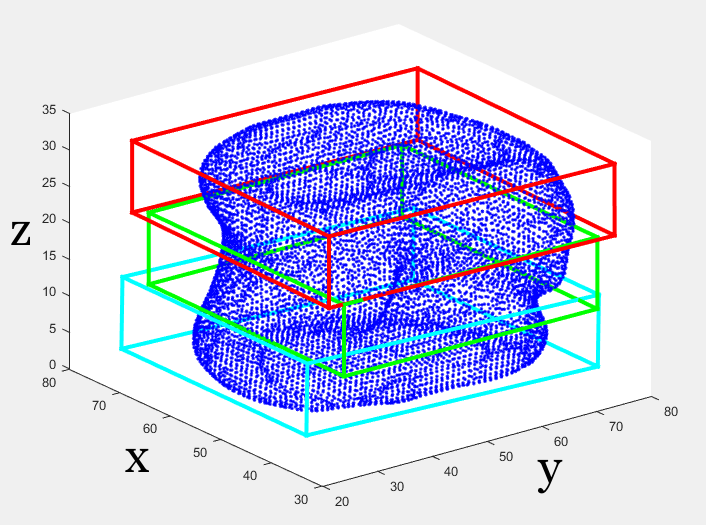
\includegraphics[width=4in]{Chapters/Chapter_PCA_images/Cuboid_fit_axial.png}
  \caption{The three cuboids fitted to the vertebra point cloud in the axial plane.}
  \label{fig:cuboid_ax}
\end{figure}

\begin{figure}[ht!]
  \centering
  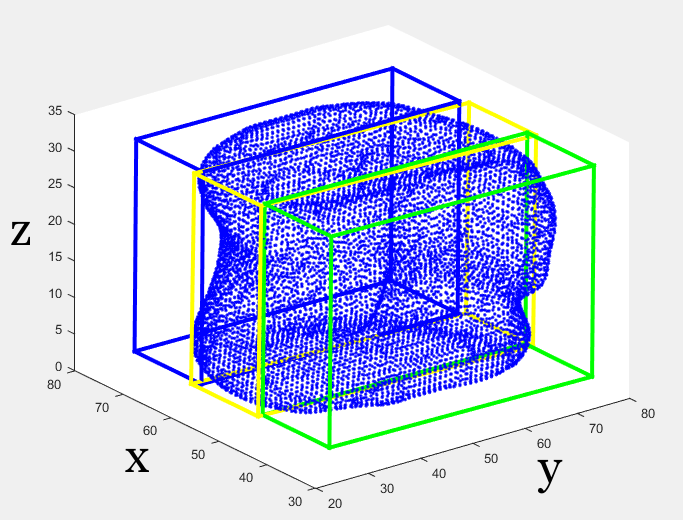
\includegraphics[width=4in]{Chapters/Chapter_PCA_images/Cuboid_fit_coronal.png}
  \caption{The three cuboids fitted to the vertebra point cloud in the coronal plane.}
  \label{fig:cuboid_cor}
\end{figure}

\begin{figure}[ht!]
  \centering
  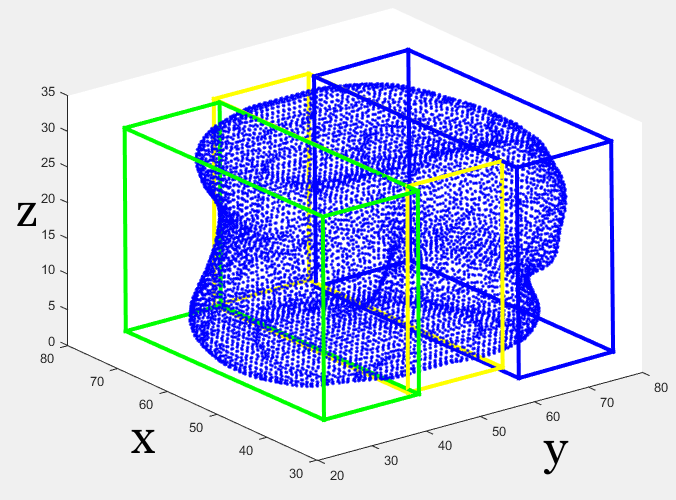
\includegraphics[width=4in]{Chapters/Chapter_PCA_images/Cuboid_fit_sagital.png}
  \caption{The three cuboids fitted to the vertebra point cloud in the sagital plane.}
  \label{fig:cuboid_sag}
\end{figure}

Measuring the two longer sides of the fitted cuboids gives a total of 18 measurements describing most aspects of the vertebral geometry, these can be seen with their abbreviations in Table \ref{tab:measurements}.
This includes identifying wedge shaped vertebrae, recorded as reduced anterior height compared to the posterior height, left to right wedge shapes, recorded as sagital left height being smaller or larger when compared to the sagital right height.

\begin{table}[ht!]
	\caption{The measurements and abbreviations taken from the vertebrae.}
	\label{tab:measurements}
	\centering
	\begin{tabular}{c|c}
    Measurement & Abbreviation \\
    \hline
    \hline
    Sagital Left Height & SLH \\
	Sagital Left Depth & SLD \\
    Sagital Mid Height & SMH \\
	Sagital Mid Depth & SMD \\
    Sagital Right Height & SRH \\
	Sagital Right Depth & SRD \\
	Coronal Anterior Height & CAH \\
	Coronal Anterior Width & CAW \\
	Coronal Mid Height & CMH \\
	Coronal Mid Width & CMW \\
	Coronal Posterior Height & CPH \\
	Coronal Posterior Width & CPW \\
	Axial Inferior Depth & AID \\
	Axial Inferior Width & AIW \\
	Axial Mid Depth & AMD \\
	Axial Mid Width & AMW \\
	Axial Superior Depth & ASD \\
	Axial Superior Width & ASW \\
	\hline
	\end{tabular}
\end{table}
\section{PCA in ScanIP}

The plugin for ScanIP that allows principal component analysis and the generation of models described by the principal components consists of five main steps.

The first of these steps is a pre-processing step, converting the masks and backgrounds into nessessary formats (.mha \& .mhd) for use with the ITK toolkit.

The following step carries out rigid registration of the models, aligning the masks and backgrounds to a shared coordinate system.
This is carried out using the ITK library with the registration being measured according to a mean squared image-to-image metric using a gradient descent optimiser. 
A limit to the number of attempts or steps allowed can be set; the default value of 100 steps for each input model was used.

The geometry of each input specimen was described in a deformable registration step, measuring the transform required to morph the mean of the input vertebrae onto each of the input vertebrae.
This step utilises the ITK FEM registration filter.

Penultimately, the transforms between the mean and each of the input vertebrae which describe the vertebral geometries are used as inputs for PCA.
Here the outputs of the step include the principal components, their eigenvalue, percentage of variation captured in that component and the cumulative percentage variation captured.

Finally, the SSAM produced can be used with the ITK Image Warp filter to generate new mask and background combinations from within the envelope of geometric and material property variation created by the input set, according to the principal components.
The plugin allows for the first five principal components to be used for as variables for model generation, altering the value of the principal components by up to three standard deviations away from the mean in both positive and negative directions.

\subsection{Generating Vertebrae Models}



\subsection{Validating Generated Vertebrae}

\subsubsection{Geometry Validation}

Measuring the vertebral geometry 18 measurements

\subsubsection{Material Property (Greyscale) Validation}

\subsubsection{Resulting Stiffness Validation}


\subsection{Measuring \& Interigating Vertebral Variation}

\subsubsection{Geometry Variation}

\subsubsection{Greyscale \& Material Property Variation}

\subsubsection{Resulting Stiffness Variation}

\section{Effect of Injected Cement Volume, Shape \& Position}



\section{Effect of Injected Cement on Vertebral Variation}
